\documentclass[hyperref=colorlinks]{beamer}
\mode<presentation>
\usetheme{iclpt}
\setbeamertemplate{navigation symbols}{}
\setbeamertemplate{headline}{
\begin{beamercolorbox}[leftskip=.2cm,rightskip=.2cm,topskip=.2cm,ht=1.1cm,dp=0.1cm,wd=\textwidth]{institute in head/foot}
  
\includegraphics[height=1cm]{icl.pdf}
  \hfill
  
\includegraphics[height=1cm]{../Pics/CMS-Color.pdf}
\end{beamercolorbox}
}
\setbeamertemplate{footline}{
\begin{beamercolorbox}[ht=.55cm,dp=0.4cm,wd=\textwidth,leftskip=.3cm]{author in head/foot}%
  \begin{minipage}[c]{5cm}%
    \usebeamerfont{author in head/foot}
    \insertshortauthor 
    \insertshorttitle
    \end{minipage}\hfill%
  \insertframenumber{} / \pageref{lastframe}
  \hfill
  \begin{minipage}{6cm}
    \hfill
  \end{minipage}
\end{beamercolorbox}%
}

\usepackage{color}
\usepackage{tabularx,colortbl}
\usepackage{graphicx}
\usepackage{pdfpages}
\usepackage{feynmp}
\DeclareGraphicsRule{*}{mps}{*}{}

\title{\vspace{-0.2cm} New Framework Overview}
%\subtitle{Paper - HIG-13-030, PASs: HIG-13-013, HIG-13-018, HIG-13-028 \vspace{-0.7cm}}
\author[P. Dunne]{\underline{P. Dunne} }%\\ on behalf of the H$\rightarrow$invisible analysis groups} % A.M. Magnan and A. Nikitenko Joao Pela with \\ R. Aggleton, J. Brooke: Bristol \\ C.Asawangtrakuldee, Q.Li: Peking \\ P. Srimanobhas: Chulalongkorn \\ S. Kumar, K. Mazumdar: Mumbai}
\titlegraphic{
  \vspace{-0.7cm}
  %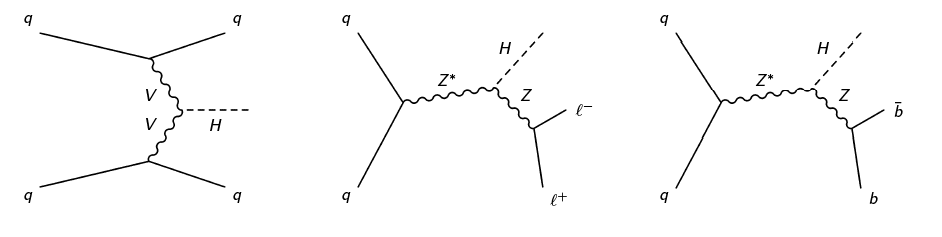
\includegraphics[width=\textwidth]{TalkPics/invcomb021213/feyndiags}
%% \begin{fmfgraph*}(100,70)
%%         \fmfleft{i1,i2}
%%         \fmfright{o1,o2,o3}
%%         \fmf{fermion}{i1,v1,o1}
%%         \fmf{fermion}{i2,v2,o3}
%%         \fmf{phantom,tension=4/5}{v1,v2}
%%         \fmffreeze
%%         \fmf{photon,label=$W,,Z$}{v1,v3}
%%         \fmf{photon,label=$W,,Z$}{v2,v3}
%%         \fmf{dashes}{v3,o2}
%%         \fmflabel{$q$}{i1}
%%         \fmflabel{$q$}{i2}
%%         \fmflabel{$q$}{o1}
%%         \fmflabel{$q$}{o3}
%%         \fmflabel{$H$}{o2}
%%       \end{fmfgraph*}
}
\date{}
\begin{document}
\begin{fmffile}{hig1330approvalfeynmandiags}

%TITLE PAGE
\section{Title}
\begin{frame}
  \titlepage
  
\end{frame}

%OUTLINE
\begin{frame}
  \frametitle{Overview}
  \begin{block}{}
    \scriptsize
    \begin{itemize}
    \item General progress update
    \item Show MVAs trained with new FW
    \item Twiki with instructions to have a go yourself can be found \href{https://twiki.cern.ch/twiki/bin/viewauth/CMS/VBFHinvisibleParkedData}{here}
    \end{itemize}
  \end{block}
\end{frame}

\begin{frame}
  \frametitle{General progress update}
  \begin{columns}
    \column{1.1\textwidth}
  \begin{block}{}
    \scriptsize
    \begin{itemize}
    \item Light trees for all samples are accessible through xrootd:
    \item[-] Some modules will run on these remotely.
    \item[-] A local copy is needed for some modules requiring access to many files at once due to xrootd memory issues.
    \item An MVA Training module is now available.
    \item Scripts to support running the framework on the Imperial and CERN batch systems have been added.
    \item Many options are now configurable through config files
    \end{itemize}
  \end{block}
  \end{columns}
\end{frame}



\begin{frame}
  \frametitle{Test of MVA Training}

  \vspace{-.3cm}

  \begin{columns}
    \column{.5\textwidth}
    \begin{block}{\scriptsize Old Macro}
      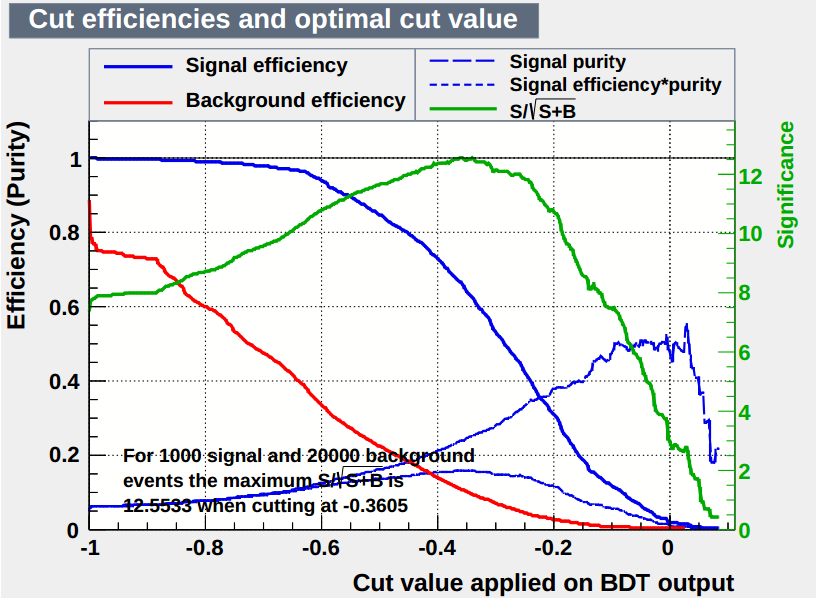
\includegraphics[width=\textwidth]{TalkPics/FWprog100614/AMbdteff.png}
    \end{block}
    \column{.5\textwidth}
    \begin{block}{\scriptsize New FW Code}
      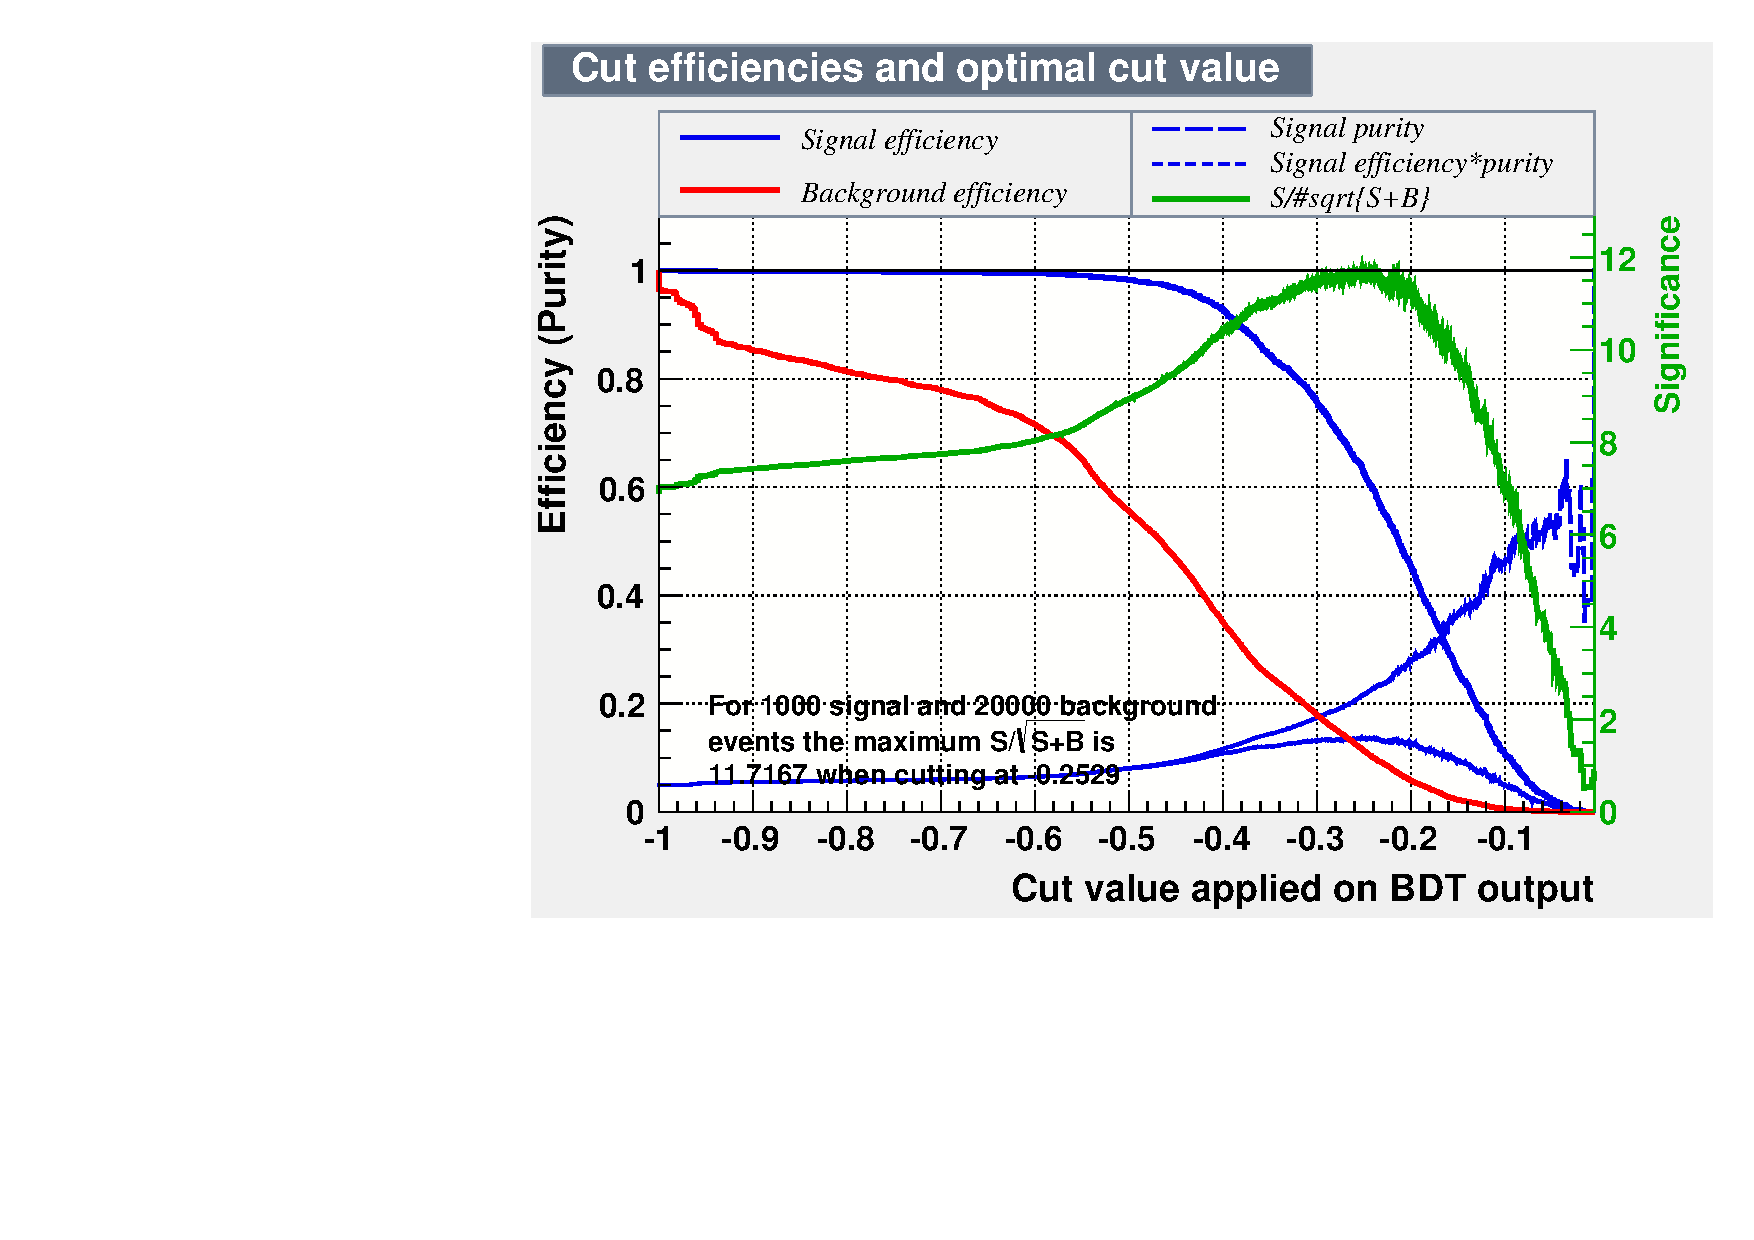
\includegraphics[width=\textwidth]{TalkPics/FWprog100614/AMrepbdteff.pdf}
    \end{block}
  \end{columns}

  \vspace{-.2cm}

  \begin{block}{}
    \scriptsize
    \begin{itemize}
    \item Same input variables and preselection
    \item Results comparable
    \item[-] Differences may be due to differing test and training tree selection
    \end{itemize}
  \end{block}

\end{frame}

\begin{frame}
  \frametitle{Instructions for new users}
  \scriptsize
  \begin{block}{}
    \begin{itemize}
    \item Follow instructions \href{https://twiki.cern.ch/twiki/bin/viewauth/CMS/VBFHinvisibleParkedData}{here} for installation
    \item A simple analysis can be found in: ICHiggsTauTau/Analysis/HiggsNuNu/LightTree/test/IntroLTAnalysis.cpp
    \item Instructions to run it can be found in  the ``For the impatient user'' section at the above link.
    \end{itemize}
  \end{block}
\end{frame}

\begin{frame}
  \frametitle{Quick Example}
  \begin{columns}
    \column{1.2\textwidth}
  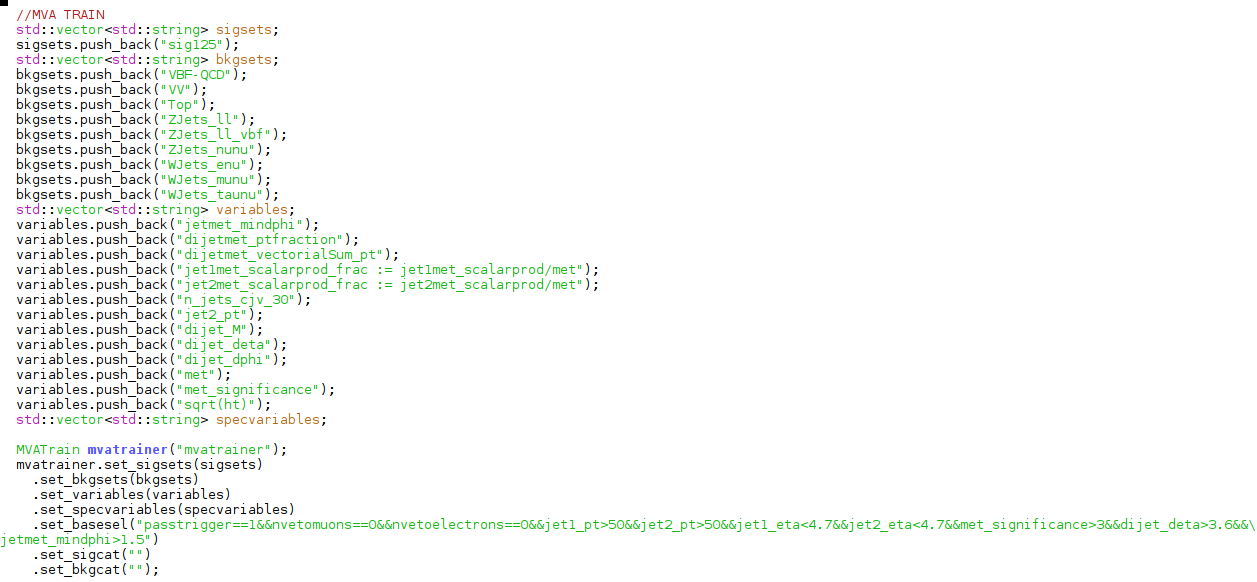
\includegraphics[height=.9\textheight]{TalkPics/FWprog100614/mvatrainsetup.png}
  \end{columns}
\end{frame}

\begin{frame}
  \frametitle{Conclusions}
  \label{lastframe}

  \begin{block}{}
    \scriptsize
    \begin{itemize}
    \item New framework now has most functionality needed for analysis optimisation
    \item[-] Instructions to try it out can be found \href{https://twiki.cern.ch/twiki/bin/viewauth/CMS/VBFHinvisibleParkedData}{here}
    \item Light Ntuples are in DCache

    \end{itemize}
  \end{block}

\end{frame}

\begin{frame}
  \frametitle{Backup}
\end{frame}


\end{fmffile}
\end{document}
